\subsection{Positional Encoding}

Employed in most models is a positional encoding operation, which adds positional information to the different input parts. Desireable features for positional encodings are the following:

\begin{itemize}
    \item The positional encoding should be unique for the positions.
    \item The positional encoding should be differentiable to be of use during training.
    \item The positional encoding should be able to extend to different input lengths outside those seen during training.
    \item The positional encoding should linearly be able to interpolate to the other encodings.
\end{itemize}

The fourth item was is inspired by Vaswani et al. in the original transformer paper where they hypothesize that models can then learn relative positions easily from such properties\cite{vaswani_attention_2017}.

There are several ways to compute the positional encoding, but a common one seen previously is the sine-cosine positional encoding, which is usually calculated as follows:

\begin{align}
    \begin{split}
        PE_{(pos, 2i)} &= \sin\left(\frac{pos}{n^{2i/d_{model}}}\right) \\
        PE_{(pos, 2i+1)} &= \cos\left(\frac{pos}{n^{2i/d_{model}}}\right)
    \end{split}
    \label{eq:pos_enc_sin}
\end{align}

In equation \ref{eq:pos_enc_sin}, $pos$ is the position of the token in the sentence, $i$ is the dimension of the positional encoding, $d_{model}$ is the dimension of the model, and $n$ is usually a constant, such as $10000$ initially proposed in the transformers paper\cite{vaswani_attention_2017}.

One can think of it as a kind of "binary encoding" but with sine and cosine functions. 

Positional encodings allow the model to learn the absolute and relative position of the different words and tokens. In figure \ref{fig:penc} you can see how the encoding would look for a sample sentence.

\textbf{RoPe: Rotary Position Embeddings}

While the sinusoidal positional encoding is extremely enticing due to its simplicity and properties, another encoding was introduced by Su et al called RoPE (Rotary Position Embeddings)\cite{su_roformer_2023}.

Simple positional encoding also did not generalize really well.

RoPE is another type of positional encoding, which is instead of based on addition with the embeddings prior to attention mechanics, it is implemented directly in the attention mechanism itself. 

RoPe formulates another approach, where they realize that in the self attention calculation, the dot product between query and key vector, $q_m^Tk_n$, could perhaps not only enable knowledge importance but also relative positional encoding, then a equaivalent function has to be found such that:

\begin{equation}
    <f_q(x_m, m), f_k(x_n, n)> = g(x_m, x_n, m-n)
\end{equation}

Where $ m - n $ is the relative positions of input. The proposed solution is a little indepth, but the intuition is to introduce a rotational matrix for the query and key vectors. A illustrative example is shown in figure \ref{fig:rope} from the paper.

\begin{figure}
    \centering
    \includegraphics[width=0.75\textwidth]{figures/RoPE.png}
    \caption{Rotary Position Embeddings; perform a rotation in plane with a constant $\theta$ scaling with the dimension.}
    \label{fig:rope}
\end{figure}

\begin{figure}
    \centering
    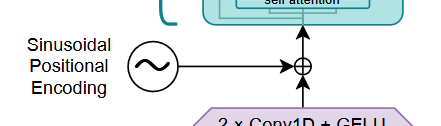
\includegraphics[width=0.75\textwidth]{figures/PosEnc.png}
    \caption{Positional encoding PLACEHOLDER}
    \label{fig:penc}
\end{figure}

\subsection{Byte Pair Encoding (BPE)}
\label{sec:bpe}

Machine Learning models working in a natural language domain require that text is parsed in a way that makes it readable for the machines. For more modern machine learning models, the pre-processing on text is usually done on huge corpi of texts. A crucial first step it is figuring out the tokenization of the input texts. Text tokenization is the discretization of words, subwords and special characters into natural numbers - including spaces and newlines. For example, the Gemma 2 9B LLM model would tokenize text "The red brown fox jumps over the lazy dog" would be tokenized into a set of discrete tokens: 

\begin{center}
    \begin{tabular}{c c c c c c c c c}
        The & \_quick & \_brown & \_fox & \_jumps & \_over & \_the & \_lazy & \_dog \\
        651 & 4320 & 8426 & 25341 & 36271 & 1163 & 573 & 27894 & 5929 \\
    \end{tabular}
\end{center}
This matches the length of our sentence, so each word (with prefixed spaces) have become their own tokens.\footnote{The tokenizer actually also produces a special token '2', which is a token specifying the "beginning of sentence".}  The tokenizer has also integrated the space (tokenized as '\_') between the words, and attached; this means that words like "hello" and " hello" - with a space - is represented as different tokens! However, what happens when a tokenizer is exposed to less common words such as some Danish words like in the sentence "Rød grød med fløde" - the following sentence would be tokenized a bit differently as can be seen below:

\begin{center}
    \begin{tabular}{c c c c c c c}
        R & ød & \_gr & ød & \_med & \_fl & øde \\
        235294 & 35173 & 2660 & 35173 & 2407 & 6067 & 100529 \\
    \end{tabular}
\end{center}

Here the words a split up  into subwords; 'grød' becomes '2434'(\_gr) and '35173'(ød) for example.

The reason for the difference lies in the algorithm used for building up the vocabulary, the \textbf{Byte Pair Encoding} which briefly will be summarised below.

\subsubsection{The algorithm}

The algorithm was initially introduced by Philip Gage in the C users manual back in 1994, the purpose of the it being "compressing" text data using a ruleset of merges to frequently occuring symbols.\cite{sennrich-etal-2016-neural}

Large Language Models all have an employed vocabulary size - larger models employ larger vocabularies. At a base level all characters receive their own unique tokens all seen in the training data.

Next the algorithm will go over the corpus and find the most common pairs of characters of length 2, and merge these into new tokens. A common example would be "th" or "he" for English, or "hv" in Danish. This will continue, next with length of 3, 4, ... and so on until the vocabulary size is reached. The algorithm is greedy, and will always merge the most common pair of tokens into a new token first based on the occurance rate.

The Byte Pair Encoding Algorithm is recursive and will also merge the new tokens into a paired token if they occur frequently as well. Say if "gr" and "ød" was both tokenied, a new token would be created for when the tokens "gr" and "ød" are seen together.

A consequence of this algorithm is of course that common words and phrases will be merged into their own tokens, leaving uncommon or rare words to be split up - potentially even down to a character level. If the corpus also don't have a lot of capitalized words compared to non-capitalized, it can also fail to split up words such as "Rød" and "rød".

This is more common for languages with low representation such as Danish.

\subsubsection{SentencePiece}

Modern LLMs do not use the original BPE algorithm as described above on its own. As shown in the examples in the beginning, tokenization also included the space character. BPE would depending on the implementatin include this, but languages are different around the world - Chinese for examples do not seperate their words with spaces.

SentencePiece is a tokenization algorithm that is language agnostic.\cite{kudo_sentencepiece_2018} It will treat the input as a raw input sequence, allowing it to be used for many languages.